\documentclass[border=3pt]{standalone}
% Shared preamble for every generated figure.
% Matches the report: newtx (Times), greyscale, square boxes.
\usepackage{newtxtext,newtxmath}
% newtx's typewriter (txtt) draws a slashed zero; use Latin Modern instead.
\renewcommand{\ttdefault}{lmtt}
\usepackage{tikz}
\usetikzlibrary{positioning,arrows.meta,calc,fit,backgrounds,shapes.geometric,
                decorations.pathreplacing,decorations.pathmorphing,matrix,patterns}

\definecolor{figgrey}{gray}{0.88}
\definecolor{figmid}{gray}{0.60}
\definecolor{figdark}{gray}{0.35}

\tikzset{
  fig/.style={font=\small},
  box/.style={draw,thick,minimum height=8mm,minimum width=22mm,align=center,
              inner sep=2pt,font=\small},
  greybox/.style={box,fill=figgrey},
  smallbox/.style={draw,minimum height=6mm,minimum width=16mm,align=center,
                   inner sep=2pt,font=\scriptsize},
  ln/.style={-{Stealth[length=2.2mm,width=1.8mm]},thick},
  lnb/.style={{Stealth[length=2.2mm,width=1.8mm]}-{Stealth[length=2.2mm,width=1.8mm]},thick},
  lbl/.style={font=\scriptsize,inner sep=1.5pt},
  note/.style={font=\scriptsize\itshape,inner sep=1.5pt},
}

\newcommand{\sline}[2]{\makebox[4mm][r]{#1}\hspace{2.5mm}\makebox[46mm][l]{\ttfamily #2}}
\newcommand{\trow}[3]{\makebox[11mm][l]{\ttfamily #1}\makebox[7mm][c]{#2}\makebox[8mm][c]{#3}}
\newcommand{\drow}[2]{\makebox[9mm][l]{\ttfamily #1}\makebox[35mm][l]{\ttfamily #2}}
\begin{document}
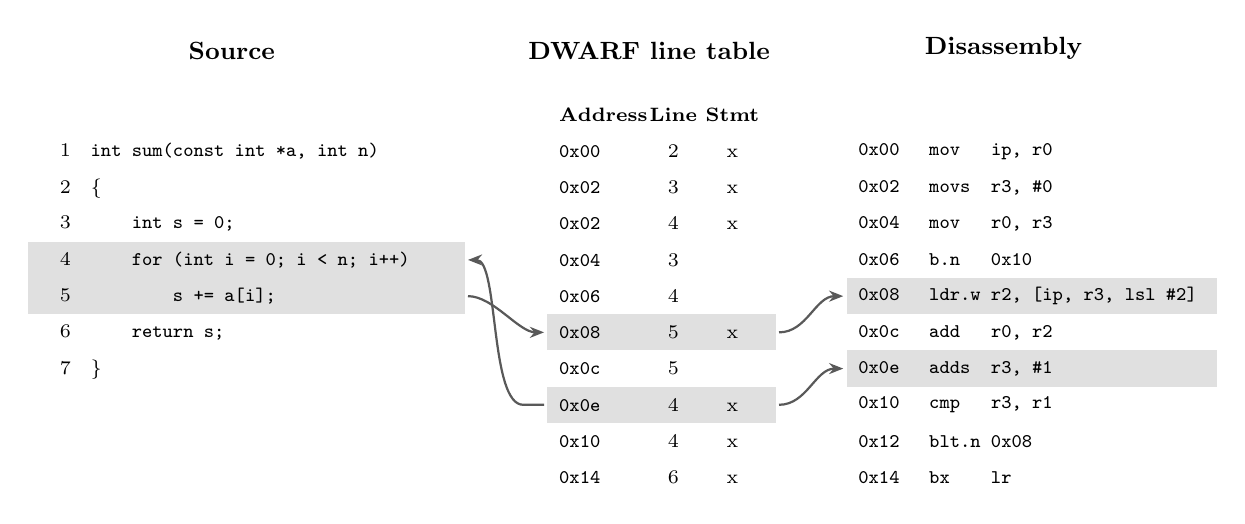
\begin{tikzpicture}[fig,
  hdr/.style={font=\small\bfseries,anchor=south},
  cellA/.style={anchor=north west,minimum height=4.6mm,font=\scriptsize,inner xsep=1.5mm},
  cellB/.style={anchor=north west,minimum height=4.6mm,font=\scriptsize,inner xsep=1.5mm},
  cellC/.style={anchor=north west,minimum height=4.6mm,font=\scriptsize,inner xsep=1.5mm},
  hl/.style={fill=figgrey},
  conn/.style={-{Stealth[length=1.8mm,width=1.4mm]},figdark,thick,shorten >=1pt,shorten <=1pt}]

\def\rh{4.6}
\def\xB{6.6}
\def\xC{10.4}

% ------------------------------------------------ column 1 : source
\node[hdr] at (2.6,0.35) {Source};
\foreach \i/\t [count=\n from 1] in {%
  1/{int sum(const int *a{,} int n)},
  2/{\{},
  3/{\ \ \ \ int s = 0;},
  4/{\ \ \ \ for (int i = 0; i < n; i++)},
  5/{\ \ \ \ \ \ \ \ s += a[i];},
  6/{\ \ \ \ return s;},
  7/{\}}}
  {\node[cellA] (s\n) at (0,-\n*\rh mm) {\sline{\i}{\t}};}
\node[cellA,hl] at (0,-4*\rh mm) {\sline{4}{\ \ \ \ for (int i = 0; i < n; i++)}};
\node[cellA,hl] (s5h) at (0,-5*\rh mm) {\sline{5}{\ \ \ \ \ \ \ \ s += a[i];}};
\node[cellA,hl] (s4h) at (0,-4*\rh mm) {\sline{4}{\ \ \ \ for (int i = 0; i < n; i++)}};

% ------------------------------------------------ column 2 : line table
\node[hdr] at (\xB+1.3,0.35) {DWARF line table};
\node[cellB] at (\xB,0) {\bfseries\makebox[11mm][l]{Address}\makebox[7mm][c]{Line}\makebox[8mm][c]{Stmt}};
\foreach \a/\l/\s [count=\n from 1] in {%
  0x00/2/x, 0x02/3/x, 0x02/4/x, 0x04/3/{}, 0x06/4/{},
  0x08/5/x, 0x0c/5/{}, 0x0e/4/x, 0x10/4/x, 0x14/6/x}
  {\node[cellB] (t\n) at (\xB,-\n*\rh mm) {\trow{\a}{\l}{\s}};}
\node[cellB,hl] (t6h) at (\xB,-6*\rh mm) {\trow{0x08}{5}{x}};
\node[cellB,hl] (t8h) at (\xB,-8*\rh mm) {\trow{0x0e}{4}{x}};

% ------------------------------------------------ column 3 : disassembly
\node[hdr] at (\xC+2.0,0.35) {Disassembly};
\foreach \a/\t [count=\n from 1] in {%
  0x00/{mov\ \ \ ip, r0}, 0x02/{movs\ \ r3, \#0}, 0x04/{mov\ \ \ r0, r3},
  0x06/{b.n\ \ \ 0x10}, 0x08/{ldr.w\ r2, [ip, r3, lsl \#2]}, 0x0c/{add\ \ \ r0, r2},
  0x0e/{adds\ \ r3, \#1}, 0x10/{cmp\ \ \ r3, r1}, 0x12/{blt.n\ 0x08}, 0x14/{bx\ \ \ \ lr}}
  {\node[cellC] (d\n) at (\xC,-\n*\rh mm) {\drow{\a}{\t}};}
\node[cellC,hl] (d5h) at (\xC,-5*\rh mm) {\drow{0x08}{ldr.w\ r2, [ip, r3, lsl \#2]}};
\node[cellC,hl] (d7h) at (\xC,-7*\rh mm) {\drow{0x0e}{adds\ \ r3, \#1}};

% ------------------------------------------------ connectors
\draw[conn] (s5h.east) to[out=0,in=180,looseness=0.8] (t6h.west);
\draw[conn] (t6h.east) to[out=0,in=180] (d5h.west);
\draw[conn] (t8h.west) -- ++(-3mm,0) to[out=180,in=0,looseness=0.55] (s4h.east);
\draw[conn] (t8h.east) to[out=0,in=180] (d7h.west);

\end{tikzpicture}
\end{document}
